\section{Vue du projet}
Notre projet est découpé en plusieurs blocs: (cf Figure 1.1)\\
\begin{itemize}
\item Le programme de scan est un programe qui peut être installé sur la machine pour automatiser l'envoi des données sur notre service
\item Le backend est le coeur de la solution
\item Le site web correspond à la partie visible par l’utilisateur
\item La machine virtuelle est une installation indépendante de notre solution permettant à un utilisateur n’avoir une copie de notre solution dont il a le contrôle.
\end{itemize}

\begin{figure}[H]
  \centering
  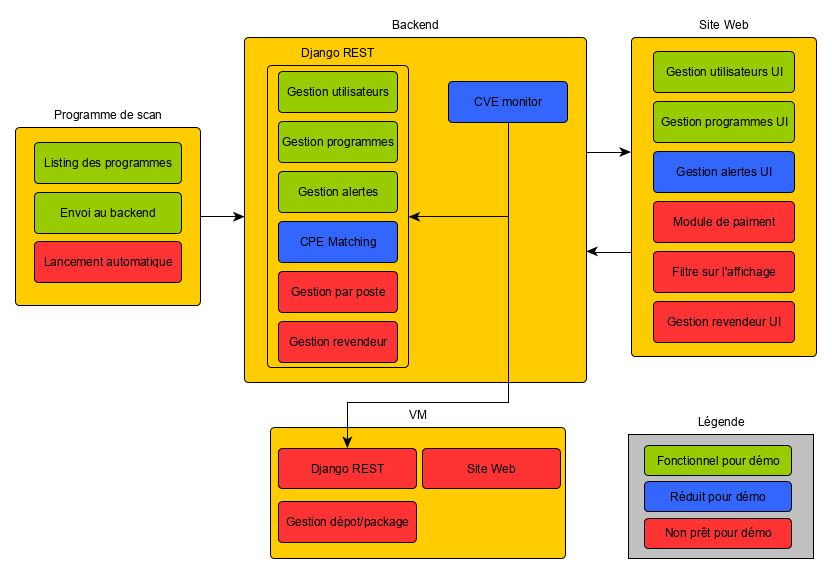
\includegraphics[width=14cm]{block_diagram.png}
  \vspace*{0.5cm}
  \caption{Vue projet}
  \vspace*{1cm}
\end{figure}

\section{Vue logique}
Sur ce schéma (Figutr 1.2), on peut voir l’interaction entre les classes principales.\\
\begin{itemize}
\item La classe Alert contient la liste des aletes actives.
\item La classe UserPrograms contient la liste des programmes sur lesquels un utilisateur veut recevoir des alertes.
\item La classe User contient les informations personnelles d’un utilisateur.
\item La classe Reference contient la liste des références utilisé par les vulnérabilitées.
\item La classe Cve contient la liste de vulnérabilité connue de notre service.
\item La classe Cpe contient la liste de programmes/version connue par notre service.
\item La classe Cwe contient la liste des descriptions de vulnérabilitée.

\end{itemize}

\begin{figure}[H]
  \centering
  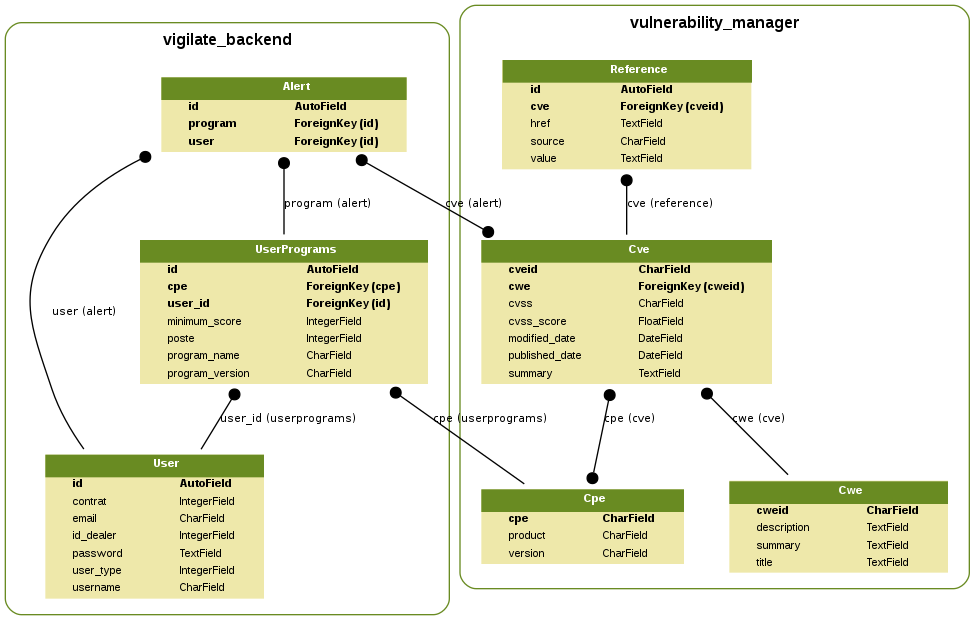
\includegraphics[width=16cm]{django_class.png}
  \vspace*{0.5cm}
  \caption{Vue Logique}
  \vspace*{1cm}
\end{figure}


\section{Norme du code}
Le langage de programmation utilisé au sein de notre solution est majoritairement python. Nous avons donc choisi de respecter la norme pep8 étant la norme recommandé pour ce langage.

\section{Tests et conditions de passage du dev à une release}
Chaque commit reçu sur le github du projet lance une suite de test d’intégration continue via travis.
Avant d’être accepté comme release, une version de dev passera par une validation via un audit de sécurité. Cet audit contiendra entre autres des test via de l’analyse static de code, des tests de scanneur web, et du fuzzing.
À partir du moment où il est décidé de fournir une release, les nouvelles features ne seront plus accepté (“freeze” de la version). En contrepartie, les issues connus et listé sur le bugtracker seront résolu afin d'augmenter la qualité du produit.
\section{Stratégie de release}
Quand une release sera prête, un tag github sera crée pour marquer cet état d’avancement.
Un exécutable windows sera crée pour le scanner de programme. (script python avec interpréteur python embarqué)
vue du projet via un schéma de haut niveau
Notre projet est découpé en plusieurs blocs:
Le site web correspond à la partie visible par l’utilisateur
Le programme de scan est un programe qui peut être installé sur la machine pour automatiser l'envoi des données sur notre service
Le backend est le coeur de la solution
La machine virtuelle est une installation indépendante de notre solution permettant à un utilisateur n’avoir une copie de notre solution dont il a le contrôle.